\newpage
\def\thoigian{90}%--Thời gian
\de{Đề số 2}{Chương V. Vectơ}

\begin{center}
	\textbf{PHẦN 1 - CÂU TRẮC NGHIỆM BỐN PHƯƠNG ÁN}
\end{center}
\Opensolutionfile{ans}[ans/ans-TN-ONTAPCHUONG-DE1]
\begin{ex}%[0H5N1-1]%[Dự án D - đợt 3 NH24-25-Hieu Phan]
	Cho tam giác $ABC$. Có thể xác định được bao nhiêu vectơ (khác vectơ-không) có điểm đầu và điểm cuối là đỉnh $A$, $B$, $C$?
	\choice
	{$2$}
	{$3$}
	{$4$}
	{\True $6$}
	\loigiai{
		Các vectơ là $\overrightarrow{AB}$, $\overrightarrow{BA}$, $\overrightarrow{AC}$,  $\overrightarrow{CA}$, $\overrightarrow{BC}$, $\overrightarrow{CB}$.
	}
\end{ex}
\begin{ex}%[0H5N1-1]%[Dự án D - đợt 3 NH24-25-Hieu Phan]
	Cho tam giác $ABC$. vectơ có điểm đầu $A$ điểm cuối $B$ là
	\choice
	{$\overrightarrow{BA}$}
	{$\overrightarrow{AC}$}
	{$\overrightarrow{BC}$}
	{\True $\overrightarrow{AB}$}
	\loigiai{vectơ có điểm đầu $A$ điểm cuối $B$ là $\overrightarrow{AB}$.}
\end{ex}
\begin{ex}%[0H5N1-3]%[Dự án D - đợt 3 NH24-25-Hieu Phan]
	Cho hình bình hành $MNPQ$. Chọn đẳng thức đúng.
	\choice
	{$\overrightarrow{MN}=\overrightarrow{PQ}$}
	{$\overrightarrow{MP}=\overrightarrow{QN}$}
	{$\overrightarrow{MQ}=\overrightarrow{PN}$}
	{\True $\overrightarrow{MN}=\overrightarrow{QP}$}
	\loigiai 
	{
		\immini 
		{
			Ta có $\overrightarrow{MN}=\overrightarrow{QP}$.
		}
		{
		\begin{tikzpicture}[line join = round,line cap = round, thick, font = \small, scale =1]
				\path 
				(0:0) coordinate (Q)
				+(0:3) coordinate (P)
				+(65:2) coordinate (M)
				($(M)+(P)-(Q)$) coordinate (N)
				;
				\draw 
				(M)--(N)--(P)--(Q)--cycle
				;
				\foreach \x/\g in {Q/-90,P/-90,M/90,N/90}
				\fill (\x) circle (1pt)
				+(\g:3mm) node{$\x$};
			\end{tikzpicture}
		}
	}
\end{ex}
\begin{ex}%[0H5N2-1]%[Dự án D - đợt 3 NH24-25-Hieu Phan]
	Cho hình bình hành $ABCD$ có $O$ là giao điểm của hai đường chéo. Khẳng định nào sau đây là đúng?
	\choice
	{$\overrightarrow{AB}=\overrightarrow{OA}-\overrightarrow{AB}$}
	{$\overrightarrow{CO}-\overrightarrow{OB}=\overrightarrow{BA}$}
	{$\overrightarrow{AB}-\overrightarrow{AD}=\overrightarrow{AC}$}
	{\True $\overrightarrow{AO}+\overrightarrow{OD}=\overrightarrow{CB}$}
	\loigiai{\immini
		{
			Ta có $\overrightarrow{AO}+\overrightarrow{OD}=\overrightarrow{AD}=\overrightarrow{CB}$, vì $ABCD$ là hình bình hành.
		}
		{
			\begin{tikzpicture}[line join = round,line cap = round, thick, font = \small, scale =1]
			\path 
			(0:0) coordinate (D)
			+(0:3) coordinate (C)
			+(65:2) coordinate (A)
			($(A)+(C)-(D)$) coordinate (B)
			;
			\draw 
			(A)--(B)--(C)--(D)--cycle
			;
			\foreach \x/\g in {D/-90,C/-90,A/90,B/90}
			\fill (\x) circle (1pt)
			+(\g:3mm) node{$\x$};
		\end{tikzpicture}
	}}
\end{ex}
\begin{ex}%[0H5N2-2]%[Dự án D - đợt 3 NH24-25-Hieu Phan]
	Cho bốn điểm bất kì $A$, $B$, $C$, $O$. Đẳng thức nào sau đây đúng?
	\choice
	{$\overrightarrow{AB}=\overrightarrow{AC}+\overrightarrow{BC}$}
	{$\overrightarrow{OA}=\overrightarrow{OB}+\overrightarrow{AB}$}
	{\True $\overrightarrow{OA}=\overrightarrow{CA}+\overrightarrow{OC}$}
	{$\overrightarrow{AB}=\overrightarrow{OB}+\overrightarrow{OA}$}
	\loigiai
	{
		Ta có $\overrightarrow{OA}=\overrightarrow{OC}+\overrightarrow{CA}=\overrightarrow{CA}+\overrightarrow{OC}$.
	}
\end{ex}
\begin{ex}%[0H5N2-4]%[Dự án D - đợt 3 NH24-25-Hieu Phan]
	Cho tam giác $ABC$ vuông tại $A$ có $AB=3$, $AC=4$. Khi đó $\left|\overrightarrow{AB}-\overrightarrow{AC}\right|$ bằng
	\choice
	{$6$}
	{$7$}
	{$1$}
	{\True $5$}
	\loigiai{
		\immini{
			Ta có $\left|\overrightarrow{AB}-\overrightarrow{AC}\right|=\left|\overrightarrow{CB}\right|=CB$.\\
			Xét tam giác $ABC$ vuông tại $A$ có $BC=\sqrt{AB^2+AC^2}=5$.\\
			Vậy $\left|\overrightarrow{AB}-\overrightarrow{AC}\right|=CB=5$.
		}
		{
			\begin{tikzpicture}[line join = round, line cap = round,>=stealth,font=\footnotesize,scale=.7]
				\foreach \x/\y/\diem in {0/0/A,4/0/C,0/3/B} \coordinate (\diem) at (\x,\y);
				\draw (A)--(B)--(C)--cycle;
				\def \dolongoc{10}
				\foreach \x/\dinh/\y in {B/A/C} \draw ($(\dinh)!\dolongoc pt!(\x)$)--($(\dinh)!\dolongoc pt!(\x)+(\dinh)!\dolongoc pt!(\y)-(\dinh)$)--($(\dinh)!\dolongoc pt!(\y)$); 
				\foreach \diem/\goc in {A/180,C/0,B/90} \fill[black](\diem) circle (1pt) ($(\diem)+(\goc:3mm)$) node{$\diem$};
			\end{tikzpicture}
		}
		
	}
\end{ex}
\begin{ex}%[0H5N3-1]%[Dự án D - đợt 3 NH24-25-Hieu Phan]
	Cho hình chữ nhật $ABCD$ có $M$, $N$ lần lượt là trung điểm của cạnh $AB$, $BC$. Giá trị $k$ thỏa mãn $\left|\overrightarrow{BD}\right|=k\left|\overrightarrow{MN}\right|$ là
	\choice
	{\True $2$}
	{$\dfrac{1}{2}$}
	{$3$}
	{$\dfrac{2}{3}$}
	\loigiai{ Ta có $M$, $N$ là đường trung bình của $\triangle ABC$ nên $\left|\overrightarrow{B D}\right|=\left|\overrightarrow{AC}\right|=2\left|\overrightarrow{M N}\right|$.\\
		Suy ra $k=2$.
	}
\end{ex}
\begin{ex}%[0H5N3-2]%[Dự án D - đợt 3 NH24-25-Hieu Phan]
	Cho $\overrightarrow{u}=2\overrightarrow{a}-3\big(\overrightarrow{a}-\overrightarrow{b}\big)+\overrightarrow{a}$. Khẳng định nào sau đây đúng?
	\choice
	{$\overrightarrow{u}=-3\overrightarrow{b}$}
	{$\overrightarrow{u}=6\overrightarrow{a}$}
	{$\overrightarrow{u}=-2\overrightarrow{a}+3\overrightarrow{b}$}
	{\True $\overrightarrow{u}=3\overrightarrow{b}$}
	\loigiai{
		Ta có $\overrightarrow{u}=2\overrightarrow{a}-3\big(\overrightarrow{a}-\overrightarrow{b}\big)+\overrightarrow{a}=2\overrightarrow{a}-3\overrightarrow{a}+3\overrightarrow{b}+\overrightarrow{a}=3\overrightarrow{b}$.
	}
\end{ex}
\begin{ex}%[0H5N3-3]%[Dự án D - đợt 3 NH24-25-Hieu Phan]
	Cho $\overrightarrow{AB}=2 \overrightarrow{AC}$. Trong các khẳng định sau, có bao nhiêu khẳng định đúng?
	\begin{enumerate}[I)]
		\item{Hai vec-tơ $\overrightarrow{AB}$,  $\overrightarrow{AC}$ cùng hướng.}
		\item{$A$, $B$, $C$ thẳng hàng và điểm $B$ nằm giữa $A$ và $C$.}
		\item{$A$, $B$, $C$ thẳng hàng và điểm $C$ nằm giữa $A$ và $B$.}
	\end{enumerate}
	\choice
	{\True $2$}
	{$1$}
	{$3$}
	{$0$}
	\loigiai{
		Ta có $\overrightarrow{AB}=2 \overrightarrow{AC}$ suy ra $C$ là trung điểm của $AB$.\\
		Vậy khẳng định I) và III) đúng.
	}
\end{ex}
\begin{ex}%[0H5N4-1]%[Dự án D - đợt 3 NH24-25-Hieu Phan]
	Cho hai vectơ $\overrightarrow{a}$ và $\overrightarrow{b}$ đều khác vectơ $\overrightarrow{0}$. Khẳng định nào sau đây đúng?
	\choice
	{$\overrightarrow{a}\cdot\overrightarrow{b}=\left|\overrightarrow{a}\right|\cdot\left|\overrightarrow{b}\right|$}
	{\True $\overrightarrow{a}\cdot\overrightarrow{b}=\left|\overrightarrow{a}\right|\cdot\left|\overrightarrow{b}\right|\cdot\cos\left(\overrightarrow{a},\overrightarrow{b}\right)$}
	{$\overrightarrow{a}\cdot\overrightarrow{b}=\left|\overrightarrow{a}\cdot\overrightarrow{b}\right|\cdot\cos\left(\overrightarrow{a},\overrightarrow{b}\right)$}
	{$\overrightarrow{a}\cdot\overrightarrow{b}=\left|\overrightarrow{a}\right|\cdot\left|\overrightarrow{b}\right|\cdot\sin\left(\overrightarrow{a},\overrightarrow{b}\right)$}
	\loigiai
	{
		Ta có $\overrightarrow{a}\cdot\overrightarrow{b}=\left|\overrightarrow{a}\right|\cdot\left|\overrightarrow{b}\right|\cdot\cos\left(\overrightarrow{a},\overrightarrow{b}\right)$.
	}
\end{ex}
\begin{ex}%[0H5H4-2]%[Dự án D - đợt 3 NH24-25-Hieu Phan]
	Cho hai vectơ có độ dài lần lượt là $3$ và $4$, tích vô hướng của hai vectơ đó là $-12$. Góc giữa hai vectơ đó bằng
	\choice
	{\True $180^{\circ}$}
	{$60^{\circ}$}
	{$90^{\circ}$}
	{$0^{\circ}$}
	\loigiai{ Gọi $\overrightarrow{a}$, $\overrightarrow{b}$ có $\heva{&\left|\overrightarrow{a}\right| = 3\\&\left|\overrightarrow{b}\right| = 4\\&\overrightarrow{a} \cdot \overrightarrow{b} = -12}$. Khi đó $\cos \left(\overrightarrow{a}, \overrightarrow{b}\right) = \dfrac{\overrightarrow{a} \cdot \overrightarrow{b}}{\left|\overrightarrow{a}\right| \cdot \left|\overrightarrow{b}\right|} = \dfrac{-12}{3 \cdot 4} = -1$.\\
		Suy ra $(\overrightarrow{a}, \overrightarrow{b}) = 180^\circ$.
	}
\end{ex}
\begin{ex}%[0H5H4-3]%[Dự án D - đợt 3 NH24-25-Hieu Phan]
	Cho tam giác $ABC$ vuông tại $A$ có $\widehat{B}=30^\circ$, $AC=2$. Gọi $M$ là trung điểm của $BC$. Tính giá trị của biểu thức $P=\overrightarrow{AM}\cdot \overrightarrow{AC}$.
	\choice
	{\True $P=2$}
	{$P=-2\sqrt{3}$}
	{$P=-2$}
	{$P=2\sqrt{3}$}
	\loigiai{
		\immini{Ta có $\overrightarrow{AM}\cdot \overrightarrow{AC}=\dfrac{1}{2}\left(\overrightarrow{AB}+\overrightarrow{AC}\right)\cdot \overrightarrow{AC}
			=\dfrac{1}{2}\overrightarrow{AB}\cdot\overrightarrow{AC}+\dfrac{1}{2}\overrightarrow{AC}^2
			=\dfrac{1}{2}AC^2=2$.}{\begin{tikzpicture}[scale=0.4,font=\footnotesize,line join = round, line cap = round, >= stealth]
				\def\x{5} \def\a{150} \def\b{90}
				\coordinate (A) at (0,0);
				\coordinate (B) at (\x,0);
				\coordinate (m) at ($(B)+(\a:1)$);
				\coordinate (n) at ($(A)+(\b:1)$);
				\coordinate (C) at (intersection of B--m and A--n);
				\coordinate (M) at ($(B)!.5!(C)$);
				\draw (A)--(B)--(C)--cycle;
				\draw (A)--(M);
				\foreach \p/\g in {A/-90,B/90,C/90,M/45} \draw[fill] (\p) circle(.5pt) node [shift={(\g:.3)}] {$\p$};
				\draw pic[draw, angle radius=3mm]{angle=C--B--A};
				\foreach \a/\b/\c in {B/A/C}
				\draw pic[draw, angle radius=2mm]{right angle=\a--\b--\c};
			\end{tikzpicture}
		}
	}
\end{ex}
\Closesolutionfile{ans}
%\begin{center}
%	\textbf{ĐÁP ÁN}
%	\inputansbox{10}{ans/ans}	
%\end{center}



\begin{center}
	\textbf{PHẦN 2 - CÂU TRẮC NGHIỆM ĐÚNG SAI}
\end{center}

\Opensolutionfile{ans}[ans/answer-DS-ONTAPCHUONG-DE1]
\setcounter{ex}{0}
\begin{ex}%[0H5V2-3]%[Dự án D - đợt 3 NH24-25-Hieu Phan]
	Cho tam giác đều $ABC$ có cạnh bằng $a$. Gọi $M$ là trung điểm của $BC$.
	\choiceTF
	{\True $\overrightarrow{AB}+\overrightarrow{BC}=a$}
	{$|\overrightarrow{AB}+\overrightarrow{AC}|=a\sqrt{2}$}
	{\True $\overrightarrow{AB}-\overrightarrow{AC}+\overrightarrow{BC}=\overrightarrow{O}$}
	{ $\overrightarrow{AM}+\overrightarrow{BM}=\overrightarrow{AB}$}
	\loigiai{
		\begin{center}
			\begin{tikzpicture}[scale=1, font=\footnotesize, line join=round, line cap=round, >=stealth]
				\draw (0,0) coordinate (A) --++(60:3) coordinate (B)--++(-60:3) coordinate (C)--(A);
				\coordinate (D) at ($(B)+(C)-(A)$);
				\path (intersection of A--D and C--B) coordinate (M);
				\draw (A)--(B)--(D)--(C) (A)--(D);
				\foreach \x/\g in {A/180,B/90,C/0,D/90,M/90}\fill[black] (\x) circle (1pt) +(\g:.3)node{$\x$};
			\end{tikzpicture}
		\end{center}
		\begin{itemchoice}
			\itemch $\overrightarrow{AB}+\overrightarrow{BC}=\overrightarrow{AC}$.
			\itemch Ta có $\overrightarrow{AB}+\overrightarrow{AC}=\overrightarrow{AD}$ (với $D$ là điểm thỏa mãn $ABDC$ là hình bình hành).\\
			Xét $\triangle ABC$, có 
			\begin{eqnarray*}
				AB^2=AM^2+BM^2
				&\Leftrightarrow&AM^2=AB^2-BM^2=AB^2-\left(\dfrac{BC}{2}\right)^2a^2-\left(\dfrac{a}{2}\right)^2=\dfrac{3a^2}{4}\\
				&\Rightarrow&AM=\dfrac{a\sqrt{3}}{2}.
			\end{eqnarray*}
			Vậy $AD=2AM=2 \cdot \dfrac{a \sqrt{3}}{2}=a\sqrt{3}$.
			\itemch Ta có $\overrightarrow{AB}-\overrightarrow{AC}+\overrightarrow{BC}= \overrightarrow{CB}+\overrightarrow{BC}= \overrightarrow{O}$.
			\itemch $\overrightarrow{AM}+\overrightarrow{BM}=\overrightarrow{AM}+\overrightarrow{MC}|=\overrightarrow{AC}$.
		\end{itemchoice}
		}
\end{ex}
\begin{ex}%[0H5H3-2]
	Cho tam giác $ABC$ có $M$, $N$, $P$ lần lượt là trung điểm của $BC$, $CA$, $AB$. Gọi $G$ là giao điểm của $AM$ và $BN$.
	\begin{center}
		\begin{tikzpicture}[scale=1.2, font=\footnotesize, line join=round, line cap=round, >=stealth]
			\def\ac{4} % cạnh AC
			\def\ab{2.5} % cạnh AB
			\def\gocA{55} % góc A của tam giác
			\coordinate[label=below left:$A$] (A) at (0,0);
			\coordinate[label=above:$B$] (B) at (\gocA:\ab);
			\coordinate[label=below right:$C$] (C) at ($(A)+(\ac,0)$);
			\coordinate[label=above right:$M$] (M) at ($(B)!0.5!(C)$);
			\coordinate[label=below:$N$] (N) at ($(A)!0.5!(C)$);
			\coordinate[label=left:$P$] (P) at ($(A)!0.5!(B)$);
			\coordinate[label=above left:$G$] (G) at ($(B)!2/3!(N)$);
			\draw (A)--(B)--(C)--(A)--(M) (B)--(N);
			\foreach \diem in {A,B,C,M,N,P,G}	\fill (\diem)circle(1pt);
		\end{tikzpicture}
	\end{center}
	\choiceTF
	{$\overrightarrow{GA}+\overrightarrow{GB}=2\overrightarrow{GC}$}
	{$\overrightarrow{AP}+\dfrac{1}{2}\overrightarrow{BC}=\overrightarrow{NA}$}
	{$\left|\overrightarrow{AG}\right|=3\left|\overrightarrow{MG}\right|$}
	{\True $\overrightarrow{MB}+\overrightarrow{MC}=\overrightarrow{0}$}
	\loigiai{
		\begin{itemchoice}
			\itemch Do $P$ là trung điểm của $AB$ nên ta có $\overrightarrow{GA}+\overrightarrow{GB}=2\overrightarrow{GP}=-\overrightarrow{GC}$.
			\itemch Ta có $PN$ là đường trung bình của $\triangle ABC \Rightarrow \overrightarrow{PN}=\dfrac{1}{2}\overrightarrow{BC}$.\\
			Do đó $\overrightarrow{AP}+\dfrac{1}{2}\overrightarrow{BC}=\overrightarrow{AP}+\overrightarrow{PN}=\overrightarrow{AN}$.
			\itemch Xét $\triangle ABC$ có $G$ là giao điểm của hai đường trung tuyến $AM$ và $BN$.\\
			Suy ra $G$ là trọng tâm của tam giác $ABC$.\\
			Khi đó $\overrightarrow{AG}=-2\overrightarrow{MG} \Rightarrow \left|\overrightarrow{AG}\right|=2\left|\overrightarrow{MG}\right|$.
			\itemch Do $M$ là trung điểm của cạnh $BC$ nên ta có $\overrightarrow{MB}+\overrightarrow{MC}=\overrightarrow{0}$.
		\end{itemchoice}
	}
\end{ex}
\Closesolutionfile{ans}
%\inputansbox[2]{2}{ans/answer.tex}



\begin{center}
\textbf{PHẦN 3 - CÂU TRẮC NGHIỆM TRẢ LỜI NGẮN}
\end{center}
\setcounter{ex}{0}
\Opensolutionfile{ans}[ans-KQ-ONTAPCHUONG-DE1]
\begin{ex}%[0H5H2-4]%[Dự án D - đợt 3 NH24-25-Hieu Phan]
	Cho hình vuông $ABCD$ có cạnh bằng $2\sqrt{5}$. Tính $\left|\overrightarrow{AB}+\overrightarrow{AC}\right|$.
	\shortans[oly]{$10$}
	\loigiai{
		\immini{
			Gọi $M$ là trung điểm $BC$, $BM = \dfrac{BC}{2} = \sqrt{5}$, khi đó $$AM = \sqrt{AB^2 + BM^2}=\sqrt{\left(2\sqrt{5}\right)^2 + \left(\sqrt{5}\right)^2} = 5.$$
			Ta có $\overrightarrow{AB} + \overrightarrow{AC} = 2\overrightarrow{AM}$ nên $\left|\overrightarrow{AB}+\overrightarrow{AC}\right| = 2AM = 10$.
		}{
			\begin{tikzpicture}[>=stealth,line join=round,line cap=round,font=\footnotesize,scale=1]
				\def\a{2}
				\path (0:0) coordinate (B)
				++(0:\a) coordinate (C)
				++(90:\a) coordinate (D)
				++(180:\a) coordinate (A)
				($(B)!.5!(C)$) coordinate (M);
				\draw (A)--(B)--(C)--(D)--cycle (A)--(M) (A)--(C);
				\foreach \x/ \goc in {A/135,B/-135,C/-45,D/45,M/-90} 
				\fill (\x) circle (1pt)
				($(\x)+(\goc:3mm)$) node {$\x$};
			\end{tikzpicture}
		}
	}
\end{ex}
\begin{ex}%[0H5V2-2]%[Dự án D - đợt 3 NH24-25-Hieu Phan]
	Cho tam giác $ABC$ có $M$ là điểm thuộc cạnh $BC$ sao cho $MB=2MC$, $N$ là trung điểm của cạnh $A C$. Giả sử $\overrightarrow{AB}=\overrightarrow{a}$, $\overrightarrow{AC}=\overrightarrow{b}$, ta có $\overrightarrow{MN}=x\overrightarrow{a}+y \overrightarrow{b}$. Khi đó tổng $3x+6y$ bằng bao nhiêu?
	\shortans[oly]{$ -2 $}
	\loigiai{
		\immini{
			Ta có $ MB=2MC \Rightarrow \overrightarrow{CM}=\dfrac{1}{3}\overrightarrow{CB}$.\\
			Khi đó
			\begin{eqnarray*}
				&\overrightarrow{MN}&=\overrightarrow{CN}-\overrightarrow{CM}\\
				& &=\dfrac{1}{2}\overrightarrow{CA}-\dfrac{1}{3}\overrightarrow{CB}\\
				& &=-\dfrac{1}{2}\overrightarrow{AC}-\dfrac{1}{3}\overrightarrow{AB}+\dfrac{1}{3}\overrightarrow{AC}\\
				& &=-\dfrac{1}{3}\overrightarrow{AB}-\dfrac{1}{6}\overrightarrow{AC}\\
				& &=-\dfrac{1}{3}\overrightarrow{a}-\dfrac{1}{6}\overrightarrow{b}.
			\end{eqnarray*}
			Nên $ x=-\dfrac{1}{3} $, $ y=-\dfrac{1}{6} $ nên $ 3x+6y=-2 $.
		}{
			\begin{tikzpicture}[scale=.8, font=\footnotesize, line join=round, line cap=round, >=stealth]
				\coordinate[label = left:$B$] (B) at (0,0);
				\coordinate[label = right:$C$] (C) at ($(B)+(6,0)$);
				\coordinate[label = above:$A$, shift=(70:4cm)] (A) at (B);
				\coordinate[label = above right:$N$] (N) at ($(A)!1/2!(C)$);
				\coordinate[label = below:$M$] (M) at ($(B)!2/3!(C)$);
				\draw (A)--(B)--(C)--cycle;
				\draw[->](M)--(N);
				\foreach \x in {A,B,C,M,N} \fill[black] (\x) circle (1.5pt);
			\end{tikzpicture}
		}
	}
\end{ex}
\begin{ex}%[0H5H4-7]%[Dự án D - đợt 3 NH24-25-Hieu Phan]
	Người ta kéo một cái thùng trượt trên sàn nhà bằng một dây hợp với phương nằm ngang một góc $60^\circ$, lực $\vec{F}$ tác dụng lên dây là $300$ N. Tính công của lực $\vec{F}$ khi thùng trượt được $15$ m.
	\begin{center}
		\begin{tikzpicture}[scale=.35,font=\footnotesize, line join=round, line cap=round, >=stealth]
			\draw (-10.4,0)--(10.4,0);
			\draw (-10,0)--($(-10,0)+(-30:1)$);
			\draw (-9,0)--($(-9,0)+(-30:1)$);
			\draw (-8,0)--($(-8,0)+(-30:1)$);
			\draw (-7,0)--($(-7,0)+(-30:1)$);
			\draw (-6,0)--($(-6,0)+(-30:1)$);
			\draw (-5,0)--($(-5,0)+(-30:1)$);
			\draw (-4,0)--($(-4,0)+(-30:1)$);
			\draw (-3,0)--($(-3,0)+(-30:1)$);
			\draw (-2,0)--($(-2,0)+(-30:1)$);
			\draw (-1,0)--($(-1,0)+(-30:1)$);
			\draw (0,0)--($(0,0)+(-30:1)$);
			\draw (1,0)--($(1,0)+(-30:1)$);
			\draw (2,0)--($(2,0)+(-30:1)$);
			\draw (3,0)--($(3,0)+(-30:1)$);
			\draw (4,0)--($(4,0)+(-30:1)$);
			\draw (5,0)--($(5,0)+(-30:1)$);
			\draw (6,0)--($(6,0)+(-30:1)$);
			\draw (7,0)--($(7,0)+(-30:1)$);
			\draw (8,0)--($(8,0)+(-30:1)$);
			\draw (9,0)--($(9,0)+(-30:1)$);
			\draw (10,0)--($(10,0)+(-30:1)$);
			\draw (3,0)--(3,2)--(-3,2)--(-3,0);
			\draw[->] (3,1)--(8,1) node[right] {$\vec{a}$};
			\draw[->] (3,1)--($(3,1)+(60:5)$) node[right] {$\vec{F}$};
			\fill (0,1) circle (2.5pt);
			\fill (3,1) circle (2.5pt);
		\end{tikzpicture} 
	\end{center}
	\shortans[oly]{$2250$}
	\loigiai{Lực kéo $\vec{F}$ hợp với phương nằm ngang một góc $60^\circ$, vật dịch chuyển theo phương nằm ngang, do đó $\left(\vec{F},\vec{a}\right)=60^\circ$.\\
		Vậy công của lực đó đã thực hiện là $A=\left|\vec{F}\right|\cdot \left|\vec{a}\right|\cdot \cos\left(\vec{F},\vec{a}\right)=300\cdot 15\cdot \cos 60^\circ=2250$ (J).
	}	
	\end{ex}
\begin{ex}%[0H5V4-1]%[Dự án D - đợt 3 NH24-25-Hieu Phan]
	Cho hình chữ nhật $ABCD$ có $AB=8$, $AD=4$. Gọi $M$ là trung điểm của cạnh $AB$, $N$ là điểm thỏa mãn $\overrightarrow{AN}=\dfrac{3}{4} \overrightarrow{AD}$. Tính $\overrightarrow{MN} \cdot \overrightarrow{AC}$.
	\shortans[oly]{$-20$}
	\loigiai{
	
		\immini
		{
			Ta có
		\allowdisplaybreaks
		\begin{eqnarray*}
			\overrightarrow{MN} \cdot \overrightarrow{AC}&=&\left(\overrightarrow{AN}-\overrightarrow{AM}\right)\cdot \overrightarrow{AC}\\
			&=&\overrightarrow{AN}\cdot \overrightarrow{AC}-\overrightarrow{AM}\cdot \overrightarrow{AC}\\
			&=&AN\cdot AC\cdot \cos\widehat{DAC}-AM\cdot AC\cdot \cos\widehat{BAC}\\
			&=&AN\cdot AC\cdot \dfrac{AD}{AC}-AM\cdot AC\cdot\dfrac{AB}{AC}\\
			&=&AN\cdot AD-AM\cdot AB\\
			&=&\dfrac{3}{4}AD^2-\dfrac{1}{2}AB^2\\
			&=&\dfrac{3}{4}\cdot 4^2-\dfrac{1}{2}\cdot 8^2\\
			&=&-20.
		\end{eqnarray*}
		}
		{
		\begin{tikzpicture}[,scale=0.6, font=\footnotesize, line join=round, line cap=round, >=stealth]
			\def\a{3}
			\path
			(0,0) coordinate (A)
			(2*\a,0) coordinate (B)
			(0,-\a) coordinate (D)
			($(D)+(B)$) coordinate (C)
			($(A)!0.5!(B)$) coordinate (M)
			($(A)!0.75!(D)$) coordinate (N)
			;
			\draw (A)--(B)--(C)--(D)--cycle (A)--(C) (M)--(N);
			\foreach \t/\g in {A/135,B/45,C/-45,D/225,M/90,N/180}{
				\draw[fill=black] (\t) circle (1pt) node[shift={(\g:9pt)},font=\scriptsize]{$ \t $};
			}
		\end{tikzpicture}
		}
	}
\end{ex}


\Closesolutionfile{ans}



\begin{center}
	\textbf{PHẦN 4 - TỰ LUẬN}
\end{center}
\setcounter{ex}{0}
\begin{ex}%[0H5V3-4]%[Dự án D - đợt 3 NH24-25-Hieu Phan]
	Cho tam giác $ABC$ có $M$ là trung điểm $BC$. Gọi $I$, $K$ là hai điểm thỏa $\overrightarrow{AI}=\dfrac{1}{3}\overrightarrow{AM},\\
	\overrightarrow{AK}=\dfrac{1}{5}\overrightarrow{AC}$. Chứng minh ba điểm $B$, $I$, $K$ thẳng hàng.
	\loigiai{
		\immini
		{
			Ta có
			\allowdisplaybreaks
			\begin{eqnarray*}
				\overrightarrow{BI}&=&\overrightarrow{BA}+\overrightarrow{AI}\\
				&=&-\overrightarrow{AB}+\dfrac{1}{3} \overrightarrow{AM} \\
				&=&-\overrightarrow{A B}+\dfrac{1}{3} \cdot \dfrac{1}{2}(\overrightarrow{A B}+\overrightarrow{AC})\\
				&=&-\dfrac{5}{6} \overrightarrow{A B}+\dfrac{1}{6} \overrightarrow{A C}.
			\end{eqnarray*}
		}
		{
			\begin{tikzpicture}[>=stealth,line join=round,line cap=round,font=\footnotesize,scale=1]
				\coordinate (B) at (0,0);
				\coordinate (C) at (3,0); \coordinate (A) at (1,2.5);
				\coordinate (M) at ($(B)!0.5!(C)$);
				\coordinate (I) at ($(A)!0.33!(M)$);
				\coordinate (K) at ($(A)!0.2!(C)$);
				\pgfresetboundingbox %Co khung hình 
				\draw (A)--(B)--(C)--cycle (I)--(B)--(K)  (A)--(M);
				\foreach \x/ \goc in {A/135,B/-135,C/-45,I/135,K/0,M/-45} 
				\fill (\x) circle (1pt)
				($(\x)+(\goc:3mm)$) node {$\x$};	   
			\end{tikzpicture}
		}
		\noindent Suy ra $6 \overrightarrow{B I}=-5 \overrightarrow{AB}+\overrightarrow{AC}.\quad(1)$\\
		Mặt khác $ \overrightarrow{BK}=\overrightarrow{AK}-\overrightarrow{AB}
		=\dfrac{1}{5} \overrightarrow{AC}-\overrightarrow{A B}$.\\
		Hay $ 5\overrightarrow{BK}=\overrightarrow{ C}-5 \overrightarrow{AB}.\quad(2)$\\
		Từ (1) và (2) suy ra $6 \overrightarrow{BI}=5 \overrightarrow{BK}$.\\
		Suy ra ba điểm $B$, $M$, $K$ thẳng hàng.
	}
\end{ex}
\begin{ex}%[0H5H3-5]%[Dự án D - đợt 3 NH24-25-Hieu Phan]
	Cho tam giác $ABC$. Gọi $M$ là trung điểm của $AB$ và $N$ là điểm trên cạnh $AC$ sao cho $NC=2NA$. Gọi $K$ là trung điểm của $MN$. Chứng minh rằng: $\overrightarrow{AK}=\dfrac{1}{4} \overrightarrow{AB}+\dfrac{1}{6} \overrightarrow{AC}$.
	\loigiai{
		\immini{Vì $K$ là trung điểm $MN$ nên 
			$$\overrightarrow{AK}=\dfrac{1}{2}\overrightarrow{AM}+\dfrac{1}{2}\overrightarrow{AN}.$$
			Vì $M$ là trung điểm $AC$ nên $\overrightarrow{AM}=\dfrac{1}{2}\overrightarrow{AB}$.\\
			Vì $NC=2NA$ và $N$ nằm trên cạnh $AC$ nên $\overrightarrow{AN}=\dfrac{1}{3}\overrightarrow{AC}$. Vậy
			$$\overrightarrow{AK}=\dfrac{1}{2}\cdot \dfrac{1}{2}\overrightarrow{AB} + \dfrac{1}{2}\cdot \dfrac{1}{3}\overrightarrow{AC} = \dfrac{1}{4} \overrightarrow{AB}+\dfrac{1}{6} \overrightarrow{AC}.$$
		}{\begin{tikzpicture}[scale=1, font=\footnotesize, line join=round, line cap=round, >=stealth]
				\path 
				(0:0) coordinate (A)
				(-1.5,-2) coordinate (B)
				(3,-2) coordinate (C);	
				\draw (A)--(B)--(C)--(A);
				\coordinate (M) at ($(A)!0.5!(B)$);
				\coordinate (N) at ($(A)!1/3!(C)$);
				\coordinate (K) at ($(M)!0.5!(N)$);
				\draw (A)--(K) (M)--(N);
				\foreach \i/\g in {A/90, B/180, C/0, M/160, N/30, K/-90}
				\fill[black](\i) circle (1pt)($(\i)+(\g:3mm)$) node{$\i$};
			\end{tikzpicture}
		}
	}
\end{ex}
\begin{ex}%[0H5V4-7]%[Dự án D - đợt 3 NH24-25-Hieu Phan]
	\immini{Cho ba lực $\overrightarrow{F}_1=\overrightarrow{MA}$, $ \overrightarrow{F}_2=\overrightarrow{MB}$, $ \overrightarrow{F}_3=\overrightarrow{MC}$ cùng tác động vào một vật tại điểm $M$ và vật đứng yên. Cho biết cường độ của $\overrightarrow{F}_1$, $\overrightarrow{F}_2$ đều bằng $30$ N và góc $\widehat{AMB}=60^\circ$. Tính cường độ lực của $\overrightarrow{F}_3$ (tham khảo hình vẽ bên).}
	{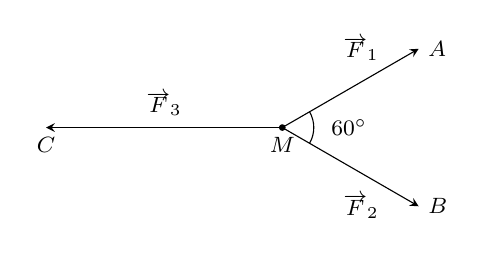
\begin{tikzpicture}[scale=1, font=\footnotesize, line join=round, line cap=round, >=stealth]
			\draw[->] (0,0)node[below]{$M$}--(-3,0)node[below]{$C$};
			\draw[->] (0,0)--([turn]120:2)node[right]{$A$};
			\draw[->] (0,0)--([turn]60:2)node[right]{$B$};
			\draw[fill=black] (0,0) circle (1pt);
			\draw (-30:4mm) arc (-30:30:4mm);
			\draw (0:5mm)node[right]{$60^\circ$};
			\draw (-1.5,0.3)node{$\overrightarrow{F}_3$}
			(1,1)node{$\overrightarrow{F}_1$}  
			(1,-1)node{$\overrightarrow{F}_2$};	
		\end{tikzpicture}
	}
	\loigiai{
		Vì ba lực cùng tác động vào điểm $M$ và vật đứng yên nên
		\allowdisplaybreaks
		\begin{eqnarray*}
		\overrightarrow{F}_1+\overrightarrow{F}_2+\overrightarrow{F}_3=\overrightarrow{0}
		&\Leftrightarrow& \overrightarrow{MA}+\overrightarrow{MB}=-\overrightarrow{MC}\\
		&\Rightarrow& \left(\overrightarrow{MA}+\overrightarrow{MB}\right)^2=\left(-\overrightarrow{MC}\right)^2\\
		&\Leftrightarrow& \overrightarrow{MA}^2+2\overrightarrow{MA}\cdot \overrightarrow{MB}+\overrightarrow{MB}^2=\overrightarrow{MC}^2\\
		&\Leftrightarrow& 30^2+2\cdot MA \cdot MB \cdot \cos\left(\overrightarrow{MA}, \overrightarrow{MB}\right)+30^2 = MC^2\\
		&\Leftrightarrow& 1800+2\cdot 30 \cdot 30 \cdot \cos 60^\circ = MC^2\\
		&\Leftrightarrow& MC^2 = 2700
		\Rightarrow MC = 30\sqrt{3}.
		\end{eqnarray*}
		Vậy cường độ lực của $\overrightarrow{F}_3$ là $30\sqrt{3}$ N.
	}
\end{ex}